\begin{figure}[htbp]
    \centering
    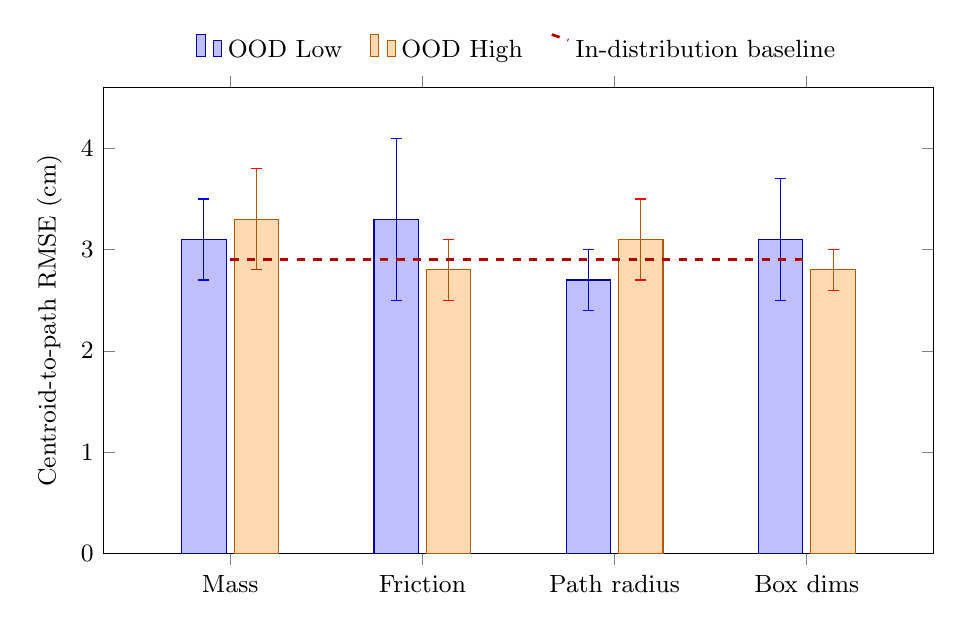
\begin{tikzpicture}
    \begin{axis}[
        ybar=3pt,
        bar width=16pt,
        width=\textwidth, height=7.5cm,
        enlarge x limits=0.22,
        ymin=0, ymax=4.6,
        ylabel={Centroid-to-path RMSE (cm)},
        symbolic x coords={Mass, Friction, Path radius, Box dims},
        xtick={Mass, Friction, Path radius, Box dims},
        legend style={at={(0.5,1.03)}, anchor=south, legend columns=3,
                      font=\small, draw=none, /tikz/every even column/.append style={column sep=8pt}},
        error bars/y dir=both, error bars/y explicit,
        tick label style={font=\small},
        label style={font=\small},
    ]
    % OOD Low
    \addplot+[draw=blue!60!black, fill=blue!25] coordinates {
        (Mass,3.1) +- (0,0.4) (Friction,3.3) +- (0,0.8)
        (Path radius,2.7) +- (0,0.3) (Box dims,3.1) +- (0,0.6) };
    % OOD High
    \addplot+[draw=orange!70!black, fill=orange!30] coordinates {
        (Mass,3.3) +- (0,0.5) (Friction,2.8) +- (0,0.3)
        (Path radius,3.1) +- (0,0.4) (Box dims,2.8) +- (0,0.2) };
    % In-distribution baseline
    \addplot+[sharp plot, no marks, draw=red!70!black, dashed, line width=1pt,
              error bars/.style={}] coordinates {
        (Mass,2.9) (Box dims,2.9) };
    \legend{OOD Low, OOD High, In-distribution baseline}
    \end{axis}
    \end{tikzpicture}
    \caption[Parameter generalization of the pushing policy]{Bar-chart visualization of the parameter-generalization results reported in \cref{tab:pho_ood} for the pushing-heavy-objects policy. Bars show centroid-to-path RMSE under single-parameter out-of-distribution shifts; error bars denote one standard deviation. The dashed line marks the in-distribution baseline ($2.9$~cm). Tracking accuracy remains stable across all OOD conditions.}
    \label{fig:pho_ood_bars}
\end{figure}
